

\tikzset{every picture/.style={line width=0.75pt}} %set default line width to 0.75pt        

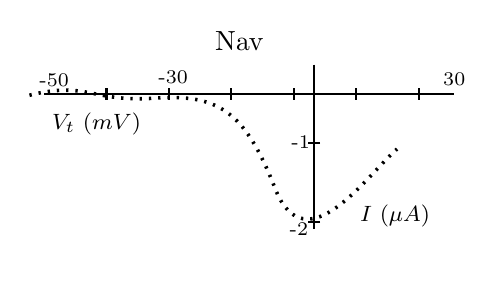
\begin{tikzpicture}[x=0.75pt,y=0.75pt,yscale=-0.7,xscale=0.7]
%uncomment if require: \path (0,300); %set diagram left start at 0, and has height of 300

%Straight Lines [id:da30256639311913547] 
\draw    (183.6,160) -- (465.5,160) (226.6,156) -- (226.6,164)(269.6,156) -- (269.6,164)(312.6,156) -- (312.6,164)(355.6,156) -- (355.6,164)(398.6,156) -- (398.6,164)(441.6,156) -- (441.6,164) ;
%Straight Lines [id:da24911735771459287] 
\draw [line width=0.75]    (369.6,139.8) -- (369.6,252.8) (373.6,193.8) -- (365.6,193.8)(373.6,247.8) -- (365.6,247.8) ;
%Curve Lines [id:da6912957926978247] 
\draw  [dash pattern={on 0.84pt off 2.51pt}] [line width=1.3] (173.6,160.8) .. controls (213.6,150.8) and (216.6,165.8) .. (259.6,162.8) .. controls (302.6,159.8) and (321.6,170.8) .. (342.6,224.8) .. controls (363.6,278.8) and (406.6,214.8) .. (426.6,197.8) ;

% Text Node
\draw (456.25,143.1) node [anchor=north west][inner sep=0.75pt]  [font=\small] [align=left] {{\scriptsize 30}};
% Text Node
\draw (360.23,193.3) node  [font=\small] [align=left] {{\scriptsize -1}};
% Text Node
\draw (367.6,252.8) node [anchor=east] [inner sep=0.75pt]  [font=\small] [align=left] {{\scriptsize -2}};
% Text Node
\draw (260.25,142.1) node [anchor=north west][inner sep=0.75pt]  [font=\small] [align=left] {{\scriptsize -30}};
% Text Node
\draw (178.25,144.1) node [anchor=north west][inner sep=0.75pt]  [font=\small] [align=left] {{\scriptsize -50}};
% Text Node
\draw (399,234) node [anchor=north west][inner sep=0.75pt]  [font=\footnotesize] [align=left] {$\displaystyle I\ ( \mu A)$};
% Text Node
\draw (187,171) node [anchor=north west][inner sep=0.75pt]  [font=\footnotesize] [align=left] {$\displaystyle V_{t} \ ( mV)$};
% Text Node
\draw (299.2,115) node [anchor=north west][inner sep=0.75pt]   [align=left] {Nav};


\end{tikzpicture}
